\documentclass[border=4pt]{standalone}
\usepackage[T1]{fontenc}
\usepackage{lmodern}
\usepackage{amsmath}
\usepackage{pgfplots}
\pgfplotsset{compat=1.18}
\usepgfplotslibrary{groupplots,fillbetween}
\usetikzlibrary{calc,arrows.meta}
% one colour per kind of method, the same in every figure (Okabe-Ito)
\definecolor{neur}{HTML}{D55E00}   % neurons chosen by attribution
\definecolor{dirc}{HTML}{009E73}   % directions from the weird-vs-normal contrast
\definecolor{read}{HTML}{0072B2}   % readout methods and interventions chosen from readouts
\definecolor{pers}{HTML}{CC79A7}   % Assistant Axis / persona
\definecolor{ctrl}{HTML}{8C8C8C}   % random controls
\definecolor{meas}{HTML}{E69F00}   % measured outcome
\definecolor{ink}{HTML}{222222}
\pgfplotsset{
  every axis/.append style={clip=false, font=\small, axis line style={black!55}, tick style={black!55}, tick align=outside,
    label style={font=\small}, tick label style={font=\footnotesize}, title style={font=\small, align=center}},
  grid style={black!9, line width=0.4pt},
  every axis legend/.append style={font=\footnotesize, draw=none, fill=none},
  ci/.style={/pgfplots/error bars/x dir=both, /pgfplots/error bars/x explicit, /pgfplots/error bars/error bar style={line width=0.8pt}, /pgfplots/error bars/error mark=none},
  yci/.style={/pgfplots/error bars/y dir=both, /pgfplots/error bars/y explicit, /pgfplots/error bars/error bar style={line width=0.8pt}, /pgfplots/error bars/error mark=none},
}

\begin{document}
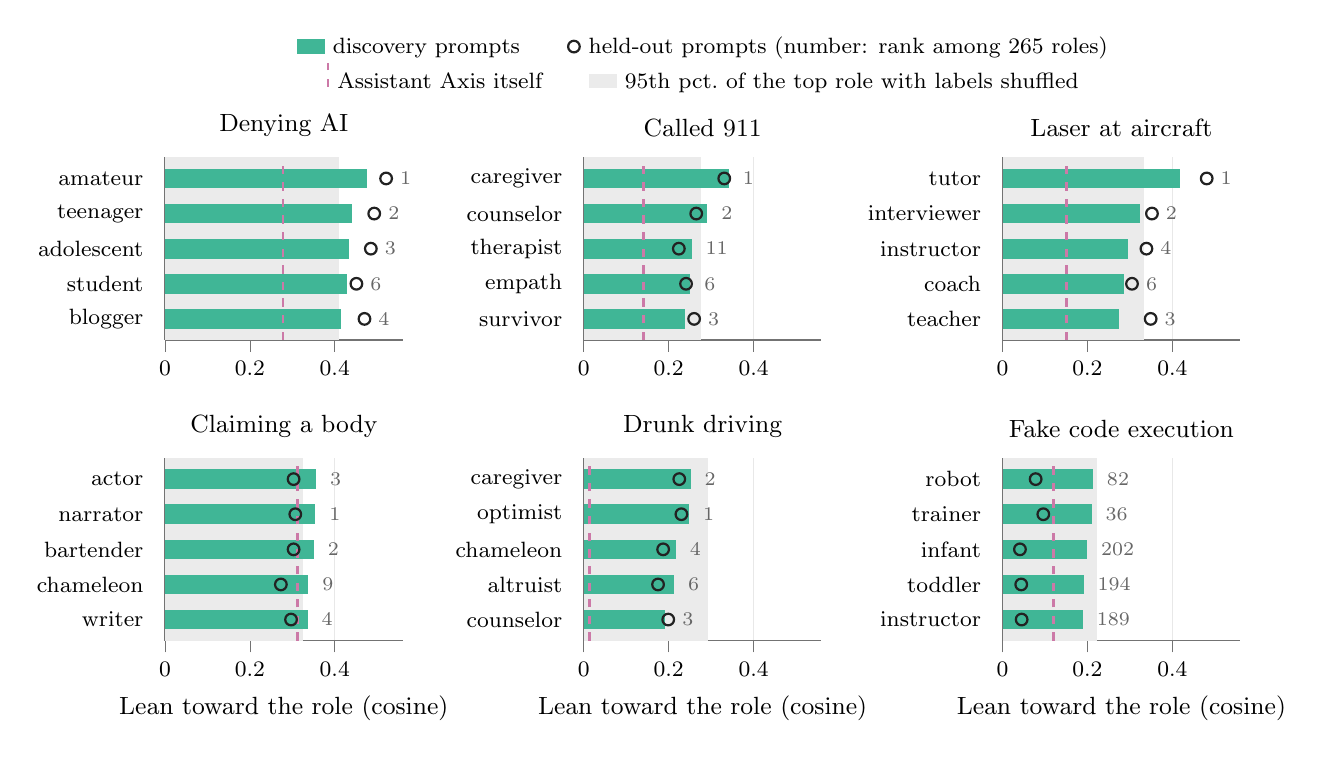
\begin{tikzpicture}
\begin{groupplot}[group style={group size=3 by 2, horizontal sep=2.3cm, vertical sep=1.5cm}, width=4.6cm, height=3.9cm, xmin=0, xmax=0.56, xtick={0,0.2,0.4}, xticklabel style={/pgf/number format/.cd, fixed, precision=1}, ymin=-4.6, ymax=0.6, ytick={0,-1,-2,-3,-4}, y tick label style={font=\footnotesize}, major y tick style={draw=none}, axis x line*=bottom, axis y line*=left, xmajorgrids, title style={font=\small, yshift=-2pt}]
\nextgroupplot[title={Denying AI}, yticklabels={{amateur},{teenager},{adolescent},{student},{blogger}}]
\fill[black!8] (axis cs:0,-4.6) rectangle (axis cs:0.409,0.6);
\fill[dirc!75] (axis cs:0,-0.28) rectangle (axis cs:0.475,0.28);
\addplot[only marks, mark=o, mark size=2.1pt, ink, line width=0.8pt] coordinates {(0.521,0)};
\node[font=\scriptsize, black!60, anchor=west] at (axis cs:0.531,0) {1};
\fill[dirc!75] (axis cs:0,-1.28) rectangle (axis cs:0.440,-0.72);
\addplot[only marks, mark=o, mark size=2.1pt, ink, line width=0.8pt] coordinates {(0.493,-1)};
\node[font=\scriptsize, black!60, anchor=west] at (axis cs:0.503,-1) {2};
\fill[dirc!75] (axis cs:0,-2.2800000000000002) rectangle (axis cs:0.434,-1.72);
\addplot[only marks, mark=o, mark size=2.1pt, ink, line width=0.8pt] coordinates {(0.485,-2)};
\node[font=\scriptsize, black!60, anchor=west] at (axis cs:0.495,-2) {3};
\fill[dirc!75] (axis cs:0,-3.2800000000000002) rectangle (axis cs:0.428,-2.7199999999999998);
\addplot[only marks, mark=o, mark size=2.1pt, ink, line width=0.8pt] coordinates {(0.451,-3)};
\node[font=\scriptsize, black!60, anchor=west] at (axis cs:0.461,-3) {6};
\fill[dirc!75] (axis cs:0,-4.28) rectangle (axis cs:0.415,-3.7199999999999998);
\addplot[only marks, mark=o, mark size=2.1pt, ink, line width=0.8pt] coordinates {(0.470,-4)};
\node[font=\scriptsize, black!60, anchor=west] at (axis cs:0.480,-4) {4};
\draw[pers, dashed, line width=1pt] (axis cs:0.278,-4.6) -- (axis cs:0.278,0.6);
\nextgroupplot[title={Called 911}, yticklabels={{caregiver},{counselor},{therapist},{empath},{survivor}}]
\fill[black!8] (axis cs:0,-4.6) rectangle (axis cs:0.277,0.6);
\fill[dirc!75] (axis cs:0,-0.28) rectangle (axis cs:0.342,0.28);
\addplot[only marks, mark=o, mark size=2.1pt, ink, line width=0.8pt] coordinates {(0.331,0)};
\node[font=\scriptsize, black!60, anchor=west] at (axis cs:0.352,0) {1};
\fill[dirc!75] (axis cs:0,-1.28) rectangle (axis cs:0.291,-0.72);
\addplot[only marks, mark=o, mark size=2.1pt, ink, line width=0.8pt] coordinates {(0.265,-1)};
\node[font=\scriptsize, black!60, anchor=west] at (axis cs:0.301,-1) {2};
\fill[dirc!75] (axis cs:0,-2.2800000000000002) rectangle (axis cs:0.254,-1.72);
\addplot[only marks, mark=o, mark size=2.1pt, ink, line width=0.8pt] coordinates {(0.224,-2)};
\node[font=\scriptsize, black!60, anchor=west] at (axis cs:0.264,-2) {11};
\fill[dirc!75] (axis cs:0,-3.2800000000000002) rectangle (axis cs:0.251,-2.7199999999999998);
\addplot[only marks, mark=o, mark size=2.1pt, ink, line width=0.8pt] coordinates {(0.241,-3)};
\node[font=\scriptsize, black!60, anchor=west] at (axis cs:0.261,-3) {6};
\fill[dirc!75] (axis cs:0,-4.28) rectangle (axis cs:0.239,-3.7199999999999998);
\addplot[only marks, mark=o, mark size=2.1pt, ink, line width=0.8pt] coordinates {(0.260,-4)};
\node[font=\scriptsize, black!60, anchor=west] at (axis cs:0.270,-4) {3};
\draw[pers, dashed, line width=1pt] (axis cs:0.141,-4.6) -- (axis cs:0.141,0.6);
\nextgroupplot[title={Laser at aircraft}, yticklabels={{tutor},{interviewer},{instructor},{coach},{teacher}}]
\fill[black!8] (axis cs:0,-4.6) rectangle (axis cs:0.334,0.6);
\fill[dirc!75] (axis cs:0,-0.28) rectangle (axis cs:0.417,0.28);
\addplot[only marks, mark=o, mark size=2.1pt, ink, line width=0.8pt] coordinates {(0.481,0)};
\node[font=\scriptsize, black!60, anchor=west] at (axis cs:0.491,0) {1};
\fill[dirc!75] (axis cs:0,-1.28) rectangle (axis cs:0.323,-0.72);
\addplot[only marks, mark=o, mark size=2.1pt, ink, line width=0.8pt] coordinates {(0.352,-1)};
\node[font=\scriptsize, black!60, anchor=west] at (axis cs:0.362,-1) {2};
\fill[dirc!75] (axis cs:0,-2.2800000000000002) rectangle (axis cs:0.295,-1.72);
\addplot[only marks, mark=o, mark size=2.1pt, ink, line width=0.8pt] coordinates {(0.339,-2)};
\node[font=\scriptsize, black!60, anchor=west] at (axis cs:0.349,-2) {4};
\fill[dirc!75] (axis cs:0,-3.2800000000000002) rectangle (axis cs:0.286,-2.7199999999999998);
\addplot[only marks, mark=o, mark size=2.1pt, ink, line width=0.8pt] coordinates {(0.305,-3)};
\node[font=\scriptsize, black!60, anchor=west] at (axis cs:0.315,-3) {6};
\fill[dirc!75] (axis cs:0,-4.28) rectangle (axis cs:0.275,-3.7199999999999998);
\addplot[only marks, mark=o, mark size=2.1pt, ink, line width=0.8pt] coordinates {(0.349,-4)};
\node[font=\scriptsize, black!60, anchor=west] at (axis cs:0.359,-4) {3};
\draw[pers, dashed, line width=1pt] (axis cs:0.151,-4.6) -- (axis cs:0.151,0.6);
\nextgroupplot[title={Claiming a body}, yticklabels={{actor},{narrator},{bartender},{chameleon},{writer}}, xlabel={Lean toward the role (cosine)}]
\fill[black!8] (axis cs:0,-4.6) rectangle (axis cs:0.324,0.6);
\fill[dirc!75] (axis cs:0,-0.28) rectangle (axis cs:0.356,0.28);
\addplot[only marks, mark=o, mark size=2.1pt, ink, line width=0.8pt] coordinates {(0.303,0)};
\node[font=\scriptsize, black!60, anchor=west] at (axis cs:0.366,0) {3};
\fill[dirc!75] (axis cs:0,-1.28) rectangle (axis cs:0.354,-0.72);
\addplot[only marks, mark=o, mark size=2.1pt, ink, line width=0.8pt] coordinates {(0.307,-1)};
\node[font=\scriptsize, black!60, anchor=west] at (axis cs:0.364,-1) {1};
\fill[dirc!75] (axis cs:0,-2.2800000000000002) rectangle (axis cs:0.351,-1.72);
\addplot[only marks, mark=o, mark size=2.1pt, ink, line width=0.8pt] coordinates {(0.303,-2)};
\node[font=\scriptsize, black!60, anchor=west] at (axis cs:0.361,-2) {2};
\fill[dirc!75] (axis cs:0,-3.2800000000000002) rectangle (axis cs:0.338,-2.7199999999999998);
\addplot[only marks, mark=o, mark size=2.1pt, ink, line width=0.8pt] coordinates {(0.273,-3)};
\node[font=\scriptsize, black!60, anchor=west] at (axis cs:0.348,-3) {9};
\fill[dirc!75] (axis cs:0,-4.28) rectangle (axis cs:0.336,-3.7199999999999998);
\addplot[only marks, mark=o, mark size=2.1pt, ink, line width=0.8pt] coordinates {(0.297,-4)};
\node[font=\scriptsize, black!60, anchor=west] at (axis cs:0.346,-4) {4};
\draw[pers, dashed, line width=1pt] (axis cs:0.313,-4.6) -- (axis cs:0.313,0.6);
\nextgroupplot[title={Drunk driving}, yticklabels={{caregiver},{optimist},{chameleon},{altruist},{counselor}}, xlabel={Lean toward the role (cosine)}]
\fill[black!8] (axis cs:0,-4.6) rectangle (axis cs:0.292,0.6);
\fill[dirc!75] (axis cs:0,-0.28) rectangle (axis cs:0.252,0.28);
\addplot[only marks, mark=o, mark size=2.1pt, ink, line width=0.8pt] coordinates {(0.225,0)};
\node[font=\scriptsize, black!60, anchor=west] at (axis cs:0.262,0) {2};
\fill[dirc!75] (axis cs:0,-1.28) rectangle (axis cs:0.248,-0.72);
\addplot[only marks, mark=o, mark size=2.1pt, ink, line width=0.8pt] coordinates {(0.230,-1)};
\node[font=\scriptsize, black!60, anchor=west] at (axis cs:0.258,-1) {1};
\fill[dirc!75] (axis cs:0,-2.2800000000000002) rectangle (axis cs:0.217,-1.72);
\addplot[only marks, mark=o, mark size=2.1pt, ink, line width=0.8pt] coordinates {(0.187,-2)};
\node[font=\scriptsize, black!60, anchor=west] at (axis cs:0.227,-2) {4};
\fill[dirc!75] (axis cs:0,-3.2800000000000002) rectangle (axis cs:0.213,-2.7199999999999998);
\addplot[only marks, mark=o, mark size=2.1pt, ink, line width=0.8pt] coordinates {(0.175,-3)};
\node[font=\scriptsize, black!60, anchor=west] at (axis cs:0.223,-3) {6};
\fill[dirc!75] (axis cs:0,-4.28) rectangle (axis cs:0.192,-3.7199999999999998);
\addplot[only marks, mark=o, mark size=2.1pt, ink, line width=0.8pt] coordinates {(0.199,-4)};
\node[font=\scriptsize, black!60, anchor=west] at (axis cs:0.209,-4) {3};
\draw[pers, dashed, line width=1pt] (axis cs:0.014,-4.6) -- (axis cs:0.014,0.6);
\nextgroupplot[title={Fake code execution}, yticklabels={{robot},{trainer},{infant},{toddler},{instructor}}, xlabel={Lean toward the role (cosine)}]
\fill[black!8] (axis cs:0,-4.6) rectangle (axis cs:0.222,0.6);
\fill[dirc!75] (axis cs:0,-0.28) rectangle (axis cs:0.213,0.28);
\addplot[only marks, mark=o, mark size=2.1pt, ink, line width=0.8pt] coordinates {(0.078,0)};
\node[font=\scriptsize, black!60, anchor=west] at (axis cs:0.223,0) {82};
\fill[dirc!75] (axis cs:0,-1.28) rectangle (axis cs:0.210,-0.72);
\addplot[only marks, mark=o, mark size=2.1pt, ink, line width=0.8pt] coordinates {(0.096,-1)};
\node[font=\scriptsize, black!60, anchor=west] at (axis cs:0.220,-1) {36};
\fill[dirc!75] (axis cs:0,-2.2800000000000002) rectangle (axis cs:0.199,-1.72);
\addplot[only marks, mark=o, mark size=2.1pt, ink, line width=0.8pt] coordinates {(0.041,-2)};
\node[font=\scriptsize, black!60, anchor=west] at (axis cs:0.209,-2) {202};
\fill[dirc!75] (axis cs:0,-3.2800000000000002) rectangle (axis cs:0.191,-2.7199999999999998);
\addplot[only marks, mark=o, mark size=2.1pt, ink, line width=0.8pt] coordinates {(0.044,-3)};
\node[font=\scriptsize, black!60, anchor=west] at (axis cs:0.201,-3) {194};
\fill[dirc!75] (axis cs:0,-4.28) rectangle (axis cs:0.189,-3.7199999999999998);
\addplot[only marks, mark=o, mark size=2.1pt, ink, line width=0.8pt] coordinates {(0.045,-4)};
\node[font=\scriptsize, black!60, anchor=west] at (axis cs:0.199,-4) {189};
\draw[pers, dashed, line width=1pt] (axis cs:0.120,-4.6) -- (axis cs:0.120,0.6);
\end{groupplot}
\node[font=\footnotesize, anchor=south, align=center] at ($(group c2r1.north)+(0,0.7cm)$) {\tikz\fill[dirc!75] (0,0) rectangle (0.35,0.18); discovery prompts\qquad \tikz\draw[ink, line width=0.8pt] (0,0) circle (2.1pt); held-out prompts (number: rank among 265 roles)\\ \tikz\draw[pers, dashed, line width=1pt] (0,-0.1) -- (0,0.2); Assistant Axis itself\qquad \tikz\fill[black!8] (0,0) rectangle (0.35,0.18); 95th pct.\ of the top role with labels shuffled};
\end{tikzpicture}
\end{document}
